\documentclass{article}
\usepackage{tikz}
\usetikzlibrary{shapes.geometric}
\usetikzlibrary{calc,positioning,shapes,arrows}
\newcommand{\Iota}{\mathcal{I}}
\tikzstyle{h} = [circle, draw, fill=white, minimum size=3em]
\tikzstyle{a} = [diamond, draw, fill=gray!40, minimum size=3em]
\tikzstyle{v} = [circle, draw, fill=gray!40, minimum size=3em]
\tikzstyle{line} = [draw, > = stealth, -latex]
\begin{document}
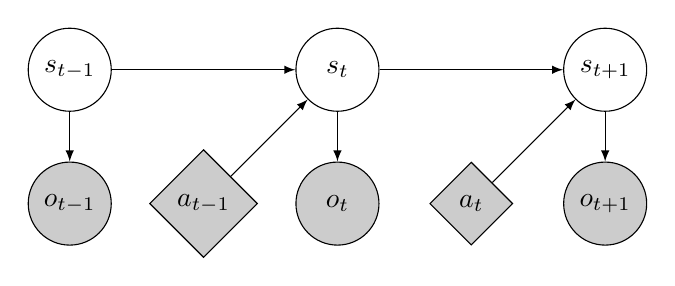
\begin{tikzpicture}[node distance = 1.7cm, auto]

%actions
\node [v] (ort) {$o_{t}$};
\node [a, right of=ort] (oht) {$a_{t}$};
\node [v, right of=oht] (ortp1) {$o_{t+1}$}; 
\node [a, left of=ort] (ohtm1) {$a_{t-1}$};
\node [v, left of=ohtm1] (ortm1) {$o_{t-1}$};
% states
\node [h, above of=ort] (st) {$s_t$}; 
\node [h, above of=ortm1] (stm1) {$s_{t-1}$}; 
\node [h, above of=ortp1] (stp1) {$s_{t+1}$}; 
% edges; state -> obs
\path [line] (st) edge (ort); 
\path [line] (stm1) edge (ortm1); 
\path [line] (stp1) edge (ortp1); 
% state -> state
\path [line] (stm1) edge (st); 
\path [line] (st) edge (stp1); 
% a -> state
\path [line] (ohtm1) edge (st); 
\path [line] (oht) edge (stp1); 
\end{tikzpicture}

\end{document}
